\section{Thiết kế, xây dựng hệ thống}

\subsection{Nền tảng và ngôn ngữ hiện thực}

\subsection{Thiết kế các cấu trúc dữ liệu}

\subsubsection{Hàng đợi ưu tiên \textit{(Priority Queue)}}

\paragraph{Mục đích sử dụng\\\\}

Quản lý hàng đợi các \textit{submission} cần được xử lý phía Server, với độ ưu tiên ở từng các \textit{submission}

\paragraph{Hiện thực\\\\}

Hình \ref{fig:class_priorityqueue} là lược đồ class của lớp PriorityQueue.

\begin{figure}[tph]
	\centering
	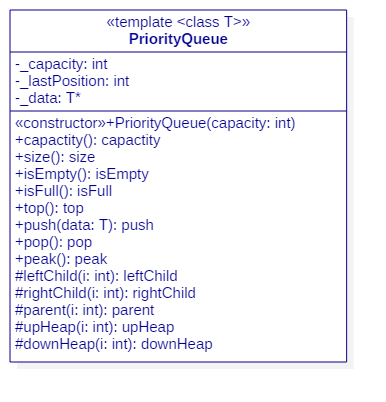
\includegraphics[width=8cm]{ClassDiagram/PriorityQueue}
	\vspace{0.3cm}
	\caption{Lược đồ class PriorityQueue}
	\label{fig:class_priorityqueue}
\end{figure}

\lstinputlisting{Code/pro-ass.xml}